% --- -----------------------------------------------------------------
% --- Elementos usados na Capa e na Folha de Rosto.
% --- EXPRESS�ES ENTRE <> DEVER�O SER COMPLETADAS COM A INFORMA��O ESPEC�FICA DO TRABALHO
% --- E OS S�MBOLOS <> DEVEM SER RETIRADOS 
% --- -----------------------------------------------------------------
\autor{MATHEUS SOUZA D'ANDREA ALVES} % deve ser escrito em maiusculo

\titulo{COLORAÇÃO DE GRAFOS$(r,\ell)$}
\instituicao{UNIVERSIDADE FEDERAL FLUMINENSE}

\orientador{Dr. Uéverton dos Santos Souza }

\local{Niterói}

\data{2018} % ano da defesa

\comentario{Trabalho de Conclusão de Curso apresentado à Universidade Federal Fluminense como requisito parcial para a obtenção do Grau
de Bacharel em Ciência da Computação.}


% --- -----------------------------------------------------------------
% --- Capa. (Capa externa, aquela com as letrinhas douradas)(Obrigatorio)
% --- ----------------------------------------------------------------
\capa

% --- -----------------------------------------------------------------
% --- Folha de rosto. (Obrigatorio)
% --- ----------------------------------------------------------------
\folhaderosto

\begin{center}
    %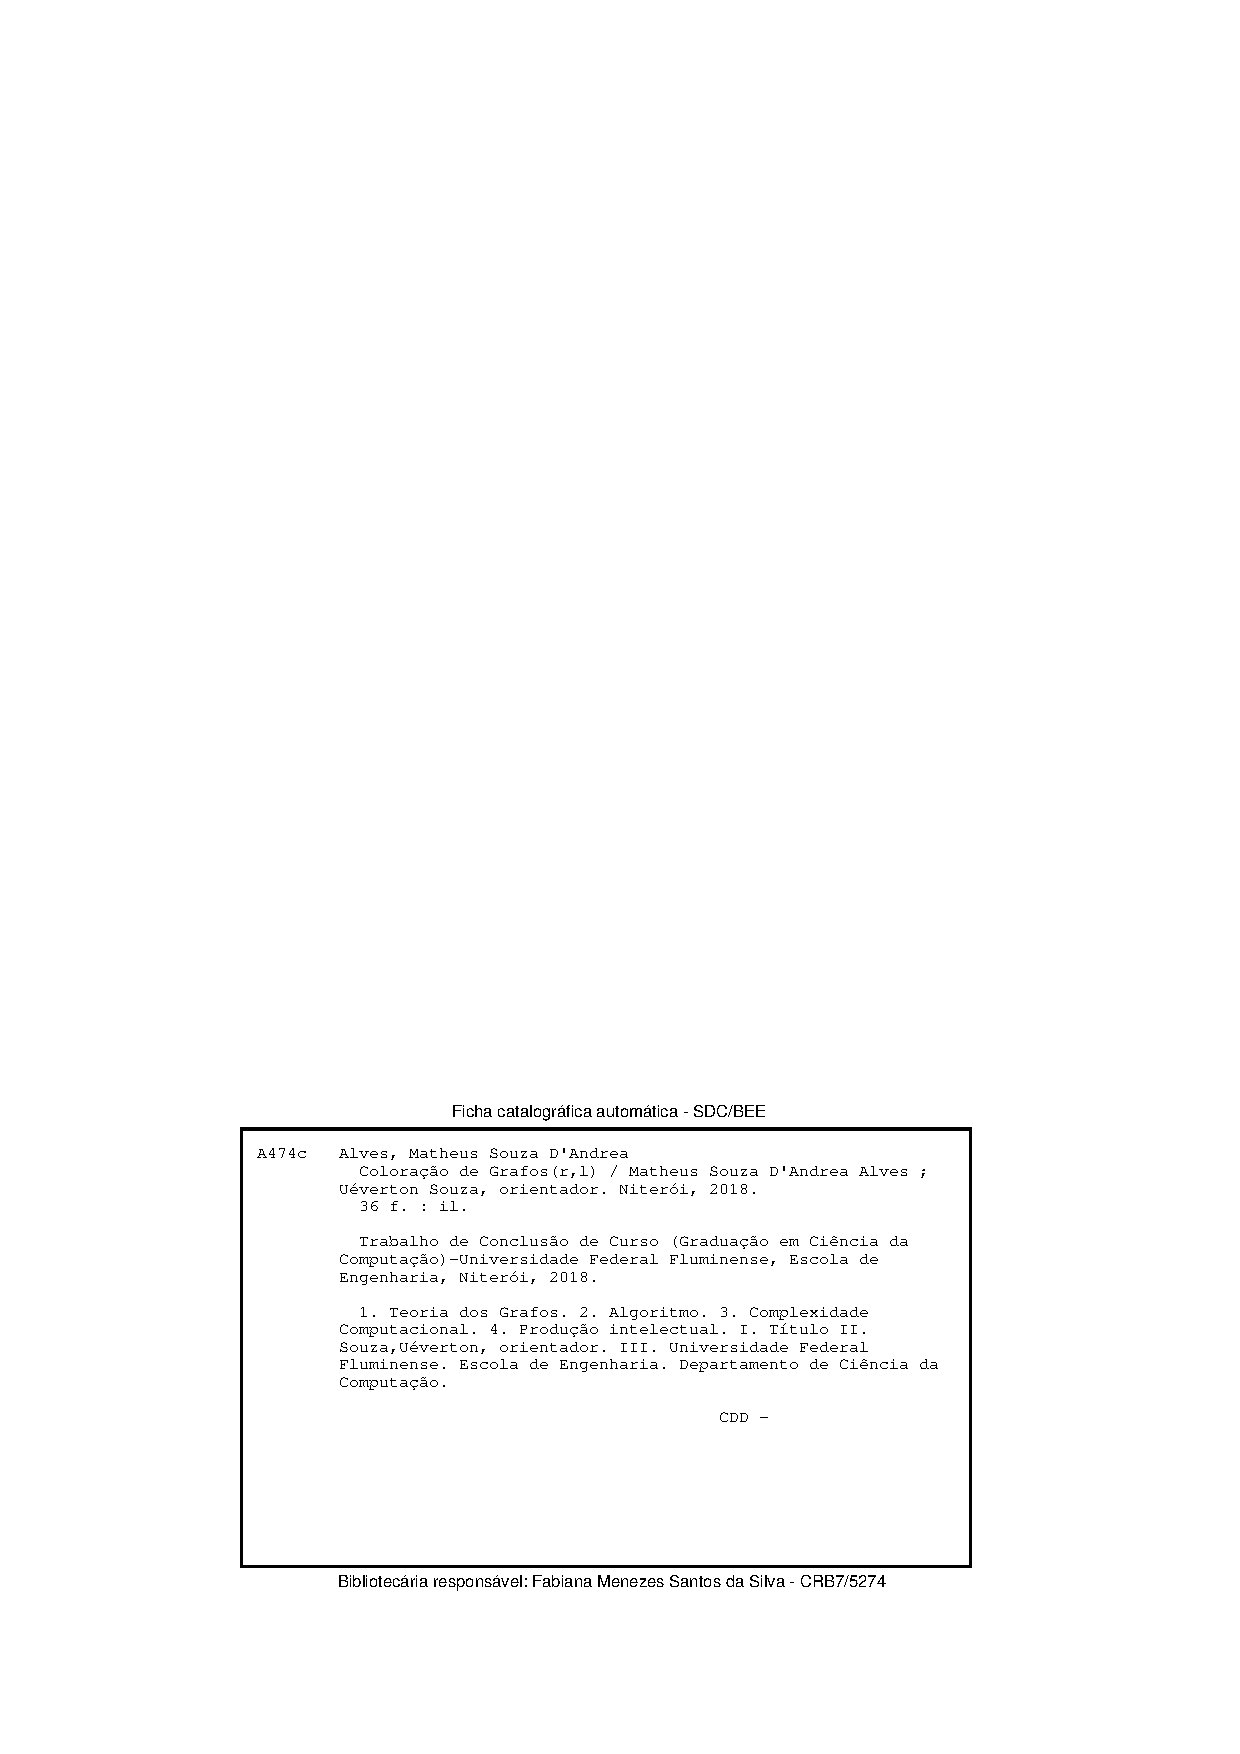
\includegraphics[scale=0.8]{ficha.pdf}    
\end{center}


\pagestyle{ruledheader}
\setcounter{page}{1}
\pagenumbering{roman}

% --- -----------------------------------------------------------------
% --- Termo de aprovacao. (Obrigatorio)
% --- ----------------------------------------------------------------
\cleardoublepage
\thispagestyle{empty}

\vspace{-60mm}

\begin{center}
   {\large MATHEUS SOUZA D'ANDREA ALVES}\\
   \vspace{7mm}
	Coloração de $Grafos(r,\ell)$\\
  \vspace{10mm}
\end{center}

\noindent
\begin{flushright}
\begin{minipage}[t]{8cm}

Trabalho de Conclusão de Curso apresentado à Universidade Federal Fluminense como requisito parcial para a obtenção do Grau
de Bacharel em Ciência da Computação.

\end{minipage}
\end{flushright}
\vspace{1.0 cm}
\noindent
Aprovada em 04/07/2018. \\ 
\begin{flushright}
   %\includegraphics[scale=0.12]{imagem/nomes.png}
\end{flushright}
\parbox{11cm}
{
 \begin{center}
BANCA EXAMINADORA \\
  \vspace{4mm}
  \rule{11cm}{.1mm} \\
    Dr. Uéverton dos Santos Souza - Orientador, UFF (Presidente)\\
    \vspace{4mm}
  \rule{11cm}{.1mm} \\
    Dr$^{\underline{a}}$. Raquel Bravo - Avaliadora, UFF\\
    \vspace{4mm}
  \rule{11cm}{.1mm} \\
    Dr$^{\underline{a}}$. Loana Tito Nogueira - Avaliadora, UFF\\
    \vspace{4mm}
  \end{center}
  }
\begin{center}
  \vspace{6mm}
  Niterói \\
  \vspace{6mm}
  2018
\end{center}

% --- -----------------------------------------------------------------
% --- Dedicatoria.(Opcional)
% --- -----------------------------------------------------------------
%\cleardoublepage
%\thispagestyle{empty}
%\vspace*{200mm}

%\begin{flushright}
%{\em 
%Dedicatoria
%}
%\end{flushright}
%\newpage


% --- -----------------------------------------------------------------
% --- Agradecimentos.(Opcional)
% --- -----------------------------------------------------------------
%\pretextualchapter{Agradecimentos}
%\hspace{5mm}
%Agradecimento

% --- -----------------------------------------------------------------
% --- Resumo em portugues.(Obrigatorio)
% --- -----------------------------------------------------------------
\begin{resumo}
	
Um problema clássico na literatura é o problema de coloração própria de um grafo, isto é, encontrar uma $q-coloração$ para um grafo $G$ tal que todo vértice $v \in V(G)$ não possua nenhum vizinho da mesma cor e $q$ seja mínimo. Esse problema é conhecido ser NP-Difícil para grafos gerais. O trabalho a seguir tem como proposta desvendar e catalogar a complexidade clássica e parametrizada de tal problema para a classe de Grafos$(r,\ell)$, i.e. grafos particionáveis em $r$ conjuntos independentes e $\ell$ cliques; Identificando as características que tornam o problema difícil e a relação do problema de coloração com outros problemas, quando abordado pela perspectiva parametrizada.

{\hspace{-8mm} \bf{Palavras-chave}}: Complexidade parametrizada. Grafos$(r,\ell)$. Partição de grafos. Coloração de Grafos

\end{resumo}

% --- -----------------------------------------------------------------
% --- Resumo em lingua estrangeira.(Obrigatorio)
% --- -----------------------------------------------------------------
\begin{abstract}

A classical problem in graph theory is the problem of proper coloring a graph, i.e. to find a $q-coloring$ for a graph $G$ such that every vertex $ v \in V (G) $ does not have any neighbor of the same color and $q$ is the smallest possible number, a problem known to be NP-Hard for a general graphs. The following work attempts to uncover and catalog the parametrized complexity of such problem for the class of graphs$(r, \ell)$, i.e. partitionable graphs in $r$ independent sets and $\ell$ cliques; Identifying the characteristics that make the problem hard and the relation of the stated problem to other problems when approached by the parameterized perspective.

{\hspace{-8mm} \bf{Keywords}}: Parametrized Complexity. Graph$(r,\ell)$. Graph Partitioning. Graph Coloring.

\end{abstract}

% --- -----------------------------------------------------------------
% --- Sumario.(Obrigatorio)
% --- -----------------------------------------------------------------
\pagestyle{ruledheader}
\listoffigures
\listoftables
\tableofcontents
